% 附录 Z：聚变堆工程——从等离子体到电网（v1.24.0 新增）
% 数值唯一来源：tools/calc/appZ_calc.py -> tools/calc/appZ_calc.txt（正文数字的唯一来源；检查项 P31）
% 单位写法：MW / MW m^-2 / kg s^-1 / g/day / GWh，全部走 \mathrm{}，不放中文字符进数学字体。
% 版权口径：只借鉴经典教材与工程文献的物理结论、公式形式与题型；文字、数值与表格自拟并独立复算。
% 本书不列 DOI，只给书名、作者、年份、卷期页。
% 分工：M 管加热与电流驱动，N 管边界与瞬态热负荷，S 管约束，U 管增益与点火，
%       V 管运行空间什么时候被撞破，W 管快粒子与 alpha 粒子，X 管辐射这条出口，
%       Y 管强场与激光等离子体；本附录管最后一环——把等离子体的功率送到电网上需要过哪几道关。

\begin{figure}[htbp]
\centering
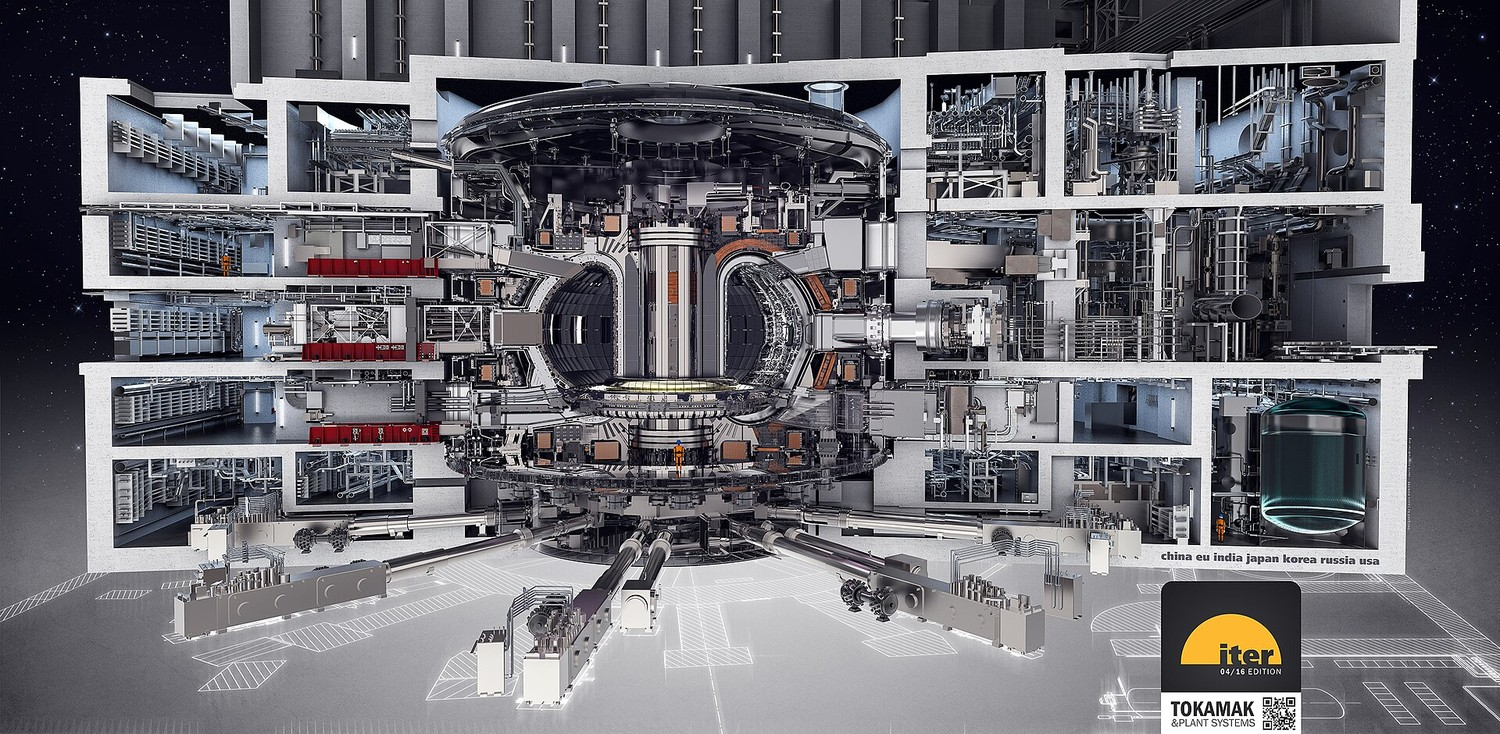
\includegraphics[width=0.72\textwidth]{../figures/iter_plant.jpg}
\caption{三本账之外：主机只是一部分。聚变堆不是一台机器，而是一座厂：磁体、真空、氚、电源、冷却与安全系统都要围着主机转。本附录的三本账（功率、中子、氚）就是这座厂能不能自持的三道门槛。}
\label{fig:photo-appz2}
\figsource{Oak Ridge National Laboratory，CC BY 2.0（Wikimedia Commons），链接见 figures/CREDITS.md。}
\end{figure}

\section{三本账接起来：从聚变功率到电功率}
\label{sec:app-z-chain}

前面每个附录只算自己那一本账：附录 U 算增益与点火，附录 W 追 alpha，附录 X 算辐射，
附录 Y 换到强场。工程上真正的验收标准只有一条：
\textbf{送出去的电，够不够抵掉自己用掉的电}。聚变功率、能量倍增、热效率、再循环份额，
四步乘完就得到净电功率。

聚变侧沿用 D1 工作点（与附录 M/S/U/V/W/X/Y 同一台装置）：$P_{\mathrm{fus}}=556.5\ \mathrm{MW}$、
$W_{\mathrm{th}}=371.4\ \mathrm{MJ}$。D-T 反应释放的 $17.6\ \mathrm{MeV}$ 按本书统一口径
分成 $1/5$ 给 alpha、$4/5$ 给中子：
\begin{equation}
P_\alpha = \frac{1}{5}P_{\mathrm{fus}} = 111.3\ \mathrm{MW},
\qquad
P_n = \frac{4}{5}P_{\mathrm{fus}} = 445.2\ \mathrm{MW}.
\label{eq:app-z-pn}
\end{equation}
（精确的能量分配是 $3.5/17.6=0.1989$ 与 $14.1/17.6=0.8011$，本书取 $1/5$ 与 $4/5$
以与附录 U/W/X 的账保持一致，误差最大 $0.57143\%$（alpha 侧）。）

中子进包层，被增殖反应与结构材料慢化，把能量放大一个因子
$M$（\textbf{声明}的量级值，铅锂包层约 $1.1$--$1.3$，本书取 $1.15$）：
\begin{equation}
P_{\mathrm{th}} = M\,P_{\mathrm{fus}} = 639.97\ \mathrm{MW},
\label{eq:app-z-pth}
\end{equation}
再经热机变成毛电功率（热效率 $\eta_{\mathrm{th}}=0.40$，\textbf{声明}值）：
\begin{equation}
P_{\mathrm{gross}} = \eta_{\mathrm{th}}P_{\mathrm{th}} = 255.99\ \mathrm{MW}.
\label{eq:app-z-pgross}
\end{equation}
但电站自己也要用电：低温系统、冷却剂泵、辅助加热、控制与磁体电源。
把这一块统一写成一个再循环份额 $f_{\mathrm{rec}}=0.15$（\textbf{声明}值），
\begin{equation}
P_{\mathrm{net}} = \left(1-f_{\mathrm{rec}}\right)P_{\mathrm{gross}}
= 217.59\ \mathrm{MW},
\qquad
\eta_{\mathrm{net}} = \frac{P_{\mathrm{net}}}{P_{\mathrm{th}}} = 0.34.
\label{eq:app-z-pnet}
\end{equation}
\textbf{$\eta_{\mathrm{net}}=0.34$ 是整条链的净效率}，它把聚变、包层、热机、
自用电四道关全乘了进去。这也是为什么「点火」只是入场券，不是终点。

把工程增益写出来，与附录 U 的 $Q$ 对照：
\begin{equation}
Q = \frac{P_{\mathrm{fus}}}{P_{\mathrm{aux}}} = 11.13,
\qquad
Q_{\mathrm{eng}} = \frac{P_{\mathrm{net}}}{P_{\mathrm{aux}}} = 4.3518,
\label{eq:app-z-qeng}
\end{equation}
其中辅助加热功率取 $P_{\mathrm{aux}}=50\ \mathrm{MW}$（\textbf{声明}值，与附录 U 同量级）。
$Q=11.13$ 而 $Q_{\mathrm{eng}}=4.3518$：\textbf{同一个堆，两个「增益」差了 $2.5575$ 倍}，
差的正是这一节乘进去的那三个因子。

\begin{table}[htbp]
\centering
\small
\caption{从聚变功率到电功率的四道关。第三列是每一关的乘子——
\textbf{任何一道关打折，后面全部按乘法缩水}，这就是工程账与等离子体账的区别。}
\label{tab:app-z-chain}
\begin{tabular}{p{3.6cm}p{3.2cm}p{3.2cm}p{3.2cm}}
\toprule
环节 & 数值 & 乘子 & 备注 \\
\midrule
聚变功率 & $556.5\ \mathrm{MW}$ & --- & D1 工作点 \\
alpha / 中子分配 & $111.3$ / $445.2\ \mathrm{MW}$ & $1/5$ 与 $4/5$ & 本书统一口径 \\
包层热功率 & $639.97\ \mathrm{MW}$ & $M = 1.15$ & 声明值 \\
毛电功率 & $255.99\ \mathrm{MW}$ & $\eta_{\mathrm{th}} = 0.40$ & 声明值 \\
净电功率 & $217.59\ \mathrm{MW}$ & $1-f_{\mathrm{rec}} = 0.85$ & 再循环 15\% \\
整链净效率 & $0.34$ & 四项相乘 & $=P_{\mathrm{net}}/P_{\mathrm{th}}$ \\
工程增益 & $Q_{\mathrm{eng}} = 4.3518$ & $P_{\mathrm{net}}/P_{\mathrm{aux}}$ & 对照 $Q = 11.13$ \\
\bottomrule
\end{tabular}

\end{table}

\begin{tip}{工程账是乘法，不是加法}{tip-app-z-chain}
等离子体物理里很多量是\textbf{相加}的（各种损失加进功率账），
工程链却几乎全是\textbf{相乘}的：$M\times\eta_{\mathrm{th}}\times(1-f_{\mathrm{rec}})$。
乘法链的坏处是「每道关都还过得去、乘积却很难看」：
$1.15\times0.40\times0.85 = 0.391$，也就是\textbf{每 $1\ \mathrm{MW}$ 聚变功率只能送出
$0.391\ \mathrm{MW}$ 电}。看到这个数，就明白为什么工程上抠每一个百分点都值得。
\end{tip}

{\footnotesize
\textbf{出处：}能量账的四步链与整链效率的定义参照 Freidberg
\emph{Plasma Physics and Fusion Energy}（2007，第 13、14 章）与 Wesson
\emph{Tokamaks}（第 4 版，2011，第 1 章）。
包层能量倍增与再循环份额的量级参照
ITER 设计报告（1999，\emph{Nucl.\ Fusion} \textbf{39}, 2137）与 Stacey
\emph{Fusion Plasma Physics}（2005，第 1 章）。本节凡标出数字的量都由
\texttt{tools/\allowbreak{}calc/\allowbreak{}appZ\_calc.py} 复算。
}

\section{中子：壁负载与材料损伤}
\label{sec:app-z-neutron}

$445.2\ \mathrm{MW}$ 的中子功率全部要穿过第一壁。第一壁只有
$A_{\mathrm{wall}}=489.532\ \mathrm{m^2}$（与附录 X 同一口径），于是\textbf{中子壁负载}
\begin{equation}
q_n = \frac{P_n}{A_{\mathrm{wall}}} = 0.90944\ \mathrm{MW\,m^{-2}}.
\label{eq:app-z-qn}
\end{equation}
工程上把 $2\ \mathrm{MW\,m^{-2}}$ 当作中子壁负载的上限（\textbf{声明}值），
本工作点的余量是 $2.1992$ 倍。这个数比想象中宽松：\textbf{难受的不是热，
而是中子把材料原子撞离格点}。位移损伤用 dpa（displacements per atom）计，
率与壁负载近似成正比（比例系数 $5\ \mathrm{dpa/year}$ 每 $\mathrm{MW\,m^{-2}}$，\textbf{声明}值）：
\begin{equation}
\dot{d} = 5\,q_n = 4.5472\ \mathrm{dpa\,year^{-1}}.
\label{eq:app-z-dpa}
\end{equation}
结构材料能承受的量级取 $50\ \mathrm{dpa}$（\textbf{声明}值），于是包层寿命
\begin{equation}
t_{\mathrm{life}} = \frac{50}{\dot d} = 10.996\ \text{年}.
\label{eq:app-z-life}
\end{equation}
\textbf{十年}。这就是聚变堆包层必须能更换的原因，也是「遥控维护」四个字的来由
（见 Z.6）。中子一年带过去的能量是 $1.4049\times10^{7}\ \mathrm{GJ}$，
相当于一座千兆瓦级电站半年的发电量：\textbf{这部分能量必须被包层收下来，
而不是让它漏到磁体上}（Z.4）。

\begin{table}[htbp]
\centering
\small
\caption{中子侧的全部关键量。第五行的 $10.996$ 年是本附录最重要的工程数字之一：
它把「材料问题」变成「维护问题」。}
\label{tab:app-z-neutron}
\begin{tabular}{p{3.4cm}p{3.0cm}p{3.4cm}p{3.3cm}}
\toprule
量 & 数值 & 由什么决定 & 含义 \\
\midrule
第一壁面积 & $489.532\ \mathrm{m^2}$ & 装置几何 & 与附录 X 同口径 \\
中子壁负载 & $0.90944\ \mathrm{MW\,m^{-2}}$ & $P_n/A_{\mathrm{wall}}$ & 上限的 $0.45472$ \\
壁负载余量 & $2.1992$ 倍 & 上限 $2\ \mathrm{MW\,m^{-2}}$ & 声明上限 \\
位移损伤率 & $4.5472\ \mathrm{dpa\,year^{-1}}$ & $5\,q_n$ & 声明系数 \\
包层寿命 & $10.996$ 年 & $50/\dot d$ & 必须可更换 \\
年输运能量 & $1.4049\times10^{7}\ \mathrm{GJ}$ & $P_n\times1$ 年 & 必须被包层收下 \\
\bottomrule
\end{tabular}

\end{table}

\begin{tip}{难受的不是热，是 dpa}{tip-app-z-neutron}
$0.90944\ \mathrm{MW\,m^{-2}}$ 的中子壁负载听起来温和。把 $445.2\ \mathrm{MW}$
摊到 $489.532\ \mathrm{m^2}$ 上而已，比附录 N 里偏滤器的稳态热流小得多。
真正的问题不在热，而在\textbf{中子把原子撞离格点}：$\dot d = 4.5472\ \mathrm{dpa\,year^{-1}}$，
$50\ \mathrm{dpa}$ 只够撑 $10.996$ 年。所以聚变堆包层是\textbf{消耗件}，
整座堆的可用率与维护方案都由这一个数决定（见 Z.6）。
\textbf{判断一个通道重不重要，要看它限制的是「功率」还是「寿命」}。
后者往往更贵。
\end{tip}

{\footnotesize
\textbf{出处：}中子壁负载与 dpa 的工程口径参照 Stacey \emph{Fusion Plasma Physics}
（2005，第 1 章）与 Atzeni \& Meyer-ter-Vehn \emph{The Physics of Inertial Fusion}
（2004，第 1 章），第一壁面积与热负荷口径与附录 N、附录 X 一致。本节数字由
\texttt{tools/\allowbreak{}calc/\allowbreak{}appZ\_calc.py} 复算。
}

\section{氚循环：增殖比、库存与自持}
\label{sec:app-z-tritium}

氚不在自然界里存货，必须\textbf{自己造}。一次 D-T 反应烧掉一个氚核、放
$17.6\ \mathrm{MeV}$，所以「每焦耳聚变能要几个氚原子」是可以直接算的：
\begin{equation}
N_T = \frac{1}{17.6\ \mathrm{MeV}} = 3.54631\times10^{11}\ \mathrm{J^{-1}},
\label{eq:app-z-burnj}
\end{equation}
乘上功率与氚原子质量 $m_T=5.00827\times10^{-27}\ \mathrm{kg}$：
\begin{equation}
\dot m_T = P_{\mathrm{fus}}N_T m_T
= 9.88393\times10^{-7}\ \mathrm{kg\,s^{-1}}
= 85.397\ \mathrm{g/day} = 31.191\ \mathrm{kg\,year^{-1}}.
\label{eq:app-z-burnrate}
\end{equation}
把它折算到「每 GW 聚变功率」是 $56.049\ \mathrm{kg\,year^{-1}}$。这个数值得记住：
\textbf{一座千兆瓦级聚变堆每年要烧掉五十多公斤氚}。

库存自己也会衰变（半衰期 $12.32$ 年，\textbf{声明}值）：衰变常数
$\lambda=\ln 2/12.32 = 0.0562619\ \mathrm{year^{-1}}$，若库存 $m_{\mathrm{inv}}=2\ \mathrm{kg}$，
\begin{equation}
\dot m_{\mathrm{decay}} = \lambda\,m_{\mathrm{inv}}
= 0.11252\ \mathrm{kg\,year^{-1}} = 0.30807\ \mathrm{g/day}.
\label{eq:app-z-decay}
\end{equation}
于是\textbf{自持}的判据可以写成一个很干净的不等式：增殖比 TBR 必须补偿
「烧掉的 + 衰变掉的」：
\begin{equation}
\mathrm{TBR}_{\min} = 1 + \frac{\dot m_{\mathrm{decay}}}{\dot m_T} = 1.0036.
\label{eq:app-z-tbrbreak}
\end{equation}
\textbf{只要 $1.0036$ 就够了}。工程上却取 $1.05$--$1.10$（本书取 $1.10$，\textbf{声明}值），
多出来的部分不是浪费，而是留给三件事：滞留、启动库存、以及增殖测量本身的误差。
净增量为
\begin{equation}
\Delta \dot m = \left(\mathrm{TBR}-1\right)\dot m_T - \dot m_{\mathrm{decay}}
= 3.0066\ \mathrm{kg\,year^{-1}}.
\label{eq:app-z-excess}
\end{equation}
最后是\textbf{处理流量}：氚不能一直待在包层里（衰变会累积、而且需要连续提取），
设处理循环时间 $\tau_{\mathrm{proc}}=4\ \mathrm{h}$，
\begin{equation}
\dot m_{\mathrm{proc}} = \frac{m_{\mathrm{inv}}}{\tau_{\mathrm{proc}}}
= 0.5\ \mathrm{kg\,h^{-1}} = 12\ \mathrm{kg/day}.
\label{eq:app-z-proc}
\end{equation}
$12\ \mathrm{kg/day}$ 的氚处理系统。这是聚变堆里唯一「每天都按公斤级搬运放射性物质」的
子系统，也是安全审查的重点。

\begin{table}[htbp]
\centering
\small
\caption{氚循环的全部关键量。第三行是最容易被忽略的一项：
\textbf{库存本身就在衰变}，所以「自持」的门槛高于 $1.000$，是 $1.0036$。}
\label{tab:app-z-tritium}
\begin{tabular}{p{3.4cm}p{3.4cm}p{3.2cm}p{3.1cm}}
\toprule
量 & 数值 & 由什么决定 & 含义 \\
\midrule
氚燃耗率 & $31.191\ \mathrm{kg\,year^{-1}}$ & $P_{\mathrm{fus}}N_Tm_T$ & $=85.397\ \mathrm{g/day}$ \\
每 GW 聚变功率 & $56.049\ \mathrm{kg\,year^{-1}}$ & 同上一行 & 记住这个数 \\
库存自衰变 & $0.11252\ \mathrm{kg\,year^{-1}}$ & $\lambda m_{\mathrm{inv}}$ & 库存 $2\ \mathrm{kg}$ \\
自持 TBR 下限 & $1.0036$ & $1+\dot m_{\mathrm{decay}}/\dot m_T$ & 只要千分之四 \\
声明 TBR & $1.10$ & 工程余量 & 净增 $3.0066\ \mathrm{kg\,year^{-1}}$ \\
处理流量 & $12\ \mathrm{kg/day}$ & $m_{\mathrm{inv}}/\tau_{\mathrm{proc}}$ & $\tau = 4\ \mathrm{h}$ \\
\bottomrule
\end{tabular}

\end{table}

\begin{tip}{自持只看两个数，余量留给不确定性}{tip-app-z-tbr}
学生常把 TBR 想成一个「越大越好」的指标。表 \ref{tab:app-z-tritium} 说明不是：
物理下限只有 $1.0036$，而工程取 $1.05$--$1.10$ 的理由\textbf{不是物理}，
而是三件事：(1) 氚会滞留在壁与包层里。
(2) 启动需要初始库存。
(3) 增殖比测量本身有误差。
\textbf{把「物理下限」与「工程余量」分开写}，是这一节唯一想留给读者的话。
把两者混成一个数，就再也说不清「为什么余量是 $10\%$ 而不是 $1\%$」。
\end{tip}

{\footnotesize
\textbf{出处：}氚燃耗与增殖比的定义参照 Freidberg \emph{Plasma Physics and Fusion
Energy}（2007，第 14 章）与 Stacey（2005，第 1 章）。
氚半衰期与衰变常数取自
NNDC/IAEA 核数据（本书不列 DOI，只给机构与量级）。
处理循环时间的量级
参照 ITER 氚系统设计报告（1999）。
}

\section{屏蔽与超导磁体：多远才够}
\label{sec:app-z-shield}

中子一旦漏到超导磁体上，后果与热负荷无关、与\textbf{超导转变温度}有关：
$4\ \mathrm{K}$ 的冷量极其昂贵。屏蔽层的衰减是指数的，衰减长度
$\lambda=0.15\ \mathrm{m}$（\textbf{声明}值，钢/水/硼体系量级），要把中子通量压到 $\varepsilon$：
\begin{equation}
x = \lambda\ln\frac{1}{\varepsilon}.
\label{eq:app-z-shield}
\end{equation}
取 $\varepsilon=10^{-6}$，得 $x = 2.0723\ \mathrm{m}$。\textbf{两米厚的屏蔽}。
漏过去的中子功率 $P_n\varepsilon = 445.2\ \mathrm{W}$，在 $4\ \mathrm{K}$ 下要付的制冷电功
（制冷系数 $\mathrm{COP}=300$，\textbf{声明}值）：
\begin{equation}
P_{\mathrm{cryo}} = \mathrm{COP}\,\varepsilon P_n = 133.56\ \mathrm{kW},
\label{eq:app-z-cryo}
\end{equation}
只占净电功率的 $0.061381\%$。\textbf{这就是「先算上限」的价值}：
做屏蔽设计之前先算漏多少、制冷要付多少，答案是「完全划得来」，
于是屏蔽的目标从「省电」变成纯粹的「保护磁体与人身安全」。

\begin{table}[htbp]
\centering
\small
\caption{屏蔽与磁体热负荷。第四行是「先算上限、再谈设计」的一个教科书式例子：
\textbf{先算出来才发现它不重要}，于是资源可以放到真正要紧的地方。}
\label{tab:app-z-shield}
\begin{tabular}{p{3.4cm}p{3.2cm}p{3.1cm}p{3.4cm}}
\toprule
量 & 数值 & 由什么决定 & 含义 \\
\midrule
衰减长度 & $0.15\ \mathrm{m}$ & 声明值 & 钢/水/硼体系量级 \\
屏蔽厚度（$10^{-6}$） & $2.0723\ \mathrm{m}$ & $\lambda\ln(1/\varepsilon)$ & 两米厚 \\
漏到磁体 & $445.2\ \mathrm{W}$ & $\varepsilon P_n$ & 作为冷负荷 \\
制冷电功 & $133.56\ \mathrm{kW}$ & $\mathrm{COP}\,\varepsilon P_n$ & 占净电 $0.061381\%$ \\
\bottomrule
\end{tabular}

\end{table}

{\footnotesize
\textbf{出处：}中子屏蔽的指数衰减与制冷系数量级参照 Stacey \emph{Fusion Plasma
Physics}（2005，第 1 章）与 Wesson \emph{Tokamaks}（第 4 版，2011，第 1 章）。
「先算上限再决定要不要细算」的做法与附录 X、附录 Y 一致。本节数字由
\texttt{tools/\allowbreak{}calc/\allowbreak{}appZ\_calc.py} 复算。
}

\section{热工与冷却剂：热怎么搬出去}
\label{sec:app-z-thermal}

$639.97\ \mathrm{MW}$ 的热必须被冷却剂带走。最简单的一步账是热量守恒：
\begin{equation}
\dot m_{\mathrm{cool}} = \frac{P_{\mathrm{th}}}{c_p\,\Delta T},
\label{eq:app-z-mdot}
\end{equation}
取氦冷却剂 $c_p = 5.2\ \mathrm{kJ\,kg^{-1}K^{-1}}$（\textbf{声明}值）、温升
$\Delta T = 200\ \mathrm{K}$（\textbf{声明}值），得
$\dot m_{\mathrm{cool}} = 615.36\ \mathrm{kg\,s^{-1}}$。\textbf{每秒六百多公斤氦}。
泵功率取热功率的 $1\%$（\textbf{声明}值）：
\begin{equation}
P_{\mathrm{pump}} = 0.01\,P_{\mathrm{th}} = 6.3997\ \mathrm{MW},
\label{eq:app-z-pump}
\end{equation}
占毛电功率的 $2.5\%$。这个数看着小，但它\textbf{已经包含在 Z.1 的再循环份额里}。
两本账必须对得上，否则就是把同一笔电算了两次。

\begin{table}[htbp]
\centering
\small
\caption{热工侧的三行账。第三行与 Z.1 的再循环份额是一回事——
\textbf{同一笔电不能在两本账里各算一次}。}
\label{tab:app-z-thermal}
\begin{tabular}{p{3.4cm}p{3.2cm}p{3.2cm}p{3.3cm}}
\toprule
量 & 数值 & 由什么决定 & 含义 \\
\midrule
冷却剂比热 & $5.2\ \mathrm{kJ\,kg^{-1}K^{-1}}$ & 声明值（氦） & 温升 $200\ \mathrm{K}$ \\
质量流量 & $615.36\ \mathrm{kg\,s^{-1}}$ & $P_{\mathrm{th}}/(c_p\Delta T)$ & 每秒六百多公斤 \\
泵功率 & $6.3997\ \mathrm{MW}$ & $0.01P_{\mathrm{th}}$ & 占毛电 $2.5\%$ \\
\bottomrule
\end{tabular}

\end{table}

\begin{tip}{两本账要对得上：泵功率在哪一边}{tip-app-z-thermal}
先算 Z.1 再算 Z.5，很容易把泵功率算两遍：一次放进 $f_{\mathrm{rec}}$，
一次又在热工账里当成「额外损失」扣掉。判别方法很简单。
\textbf{问一句「这个数最后从哪一笔电里出」}。如果它已经在 $f_{\mathrm{rec}}$ 里，
本节就只算它的\textbf{物理量级}（流量、扬程、占多少），不再从电功率里扣。
工程账最常见的错是\textbf{把同一笔钱花两次}。
\end{tip}

{\footnotesize
\textbf{出处：}热量守恒与冷却剂流量账参照 Stacey（2005，第 1 章）。
氦冷却剂的比热与温升量级参照 ITER 设计报告（1999）与 Freidberg（2007，第 14 章）。
}

\begin{figure}[htbp]
\centering
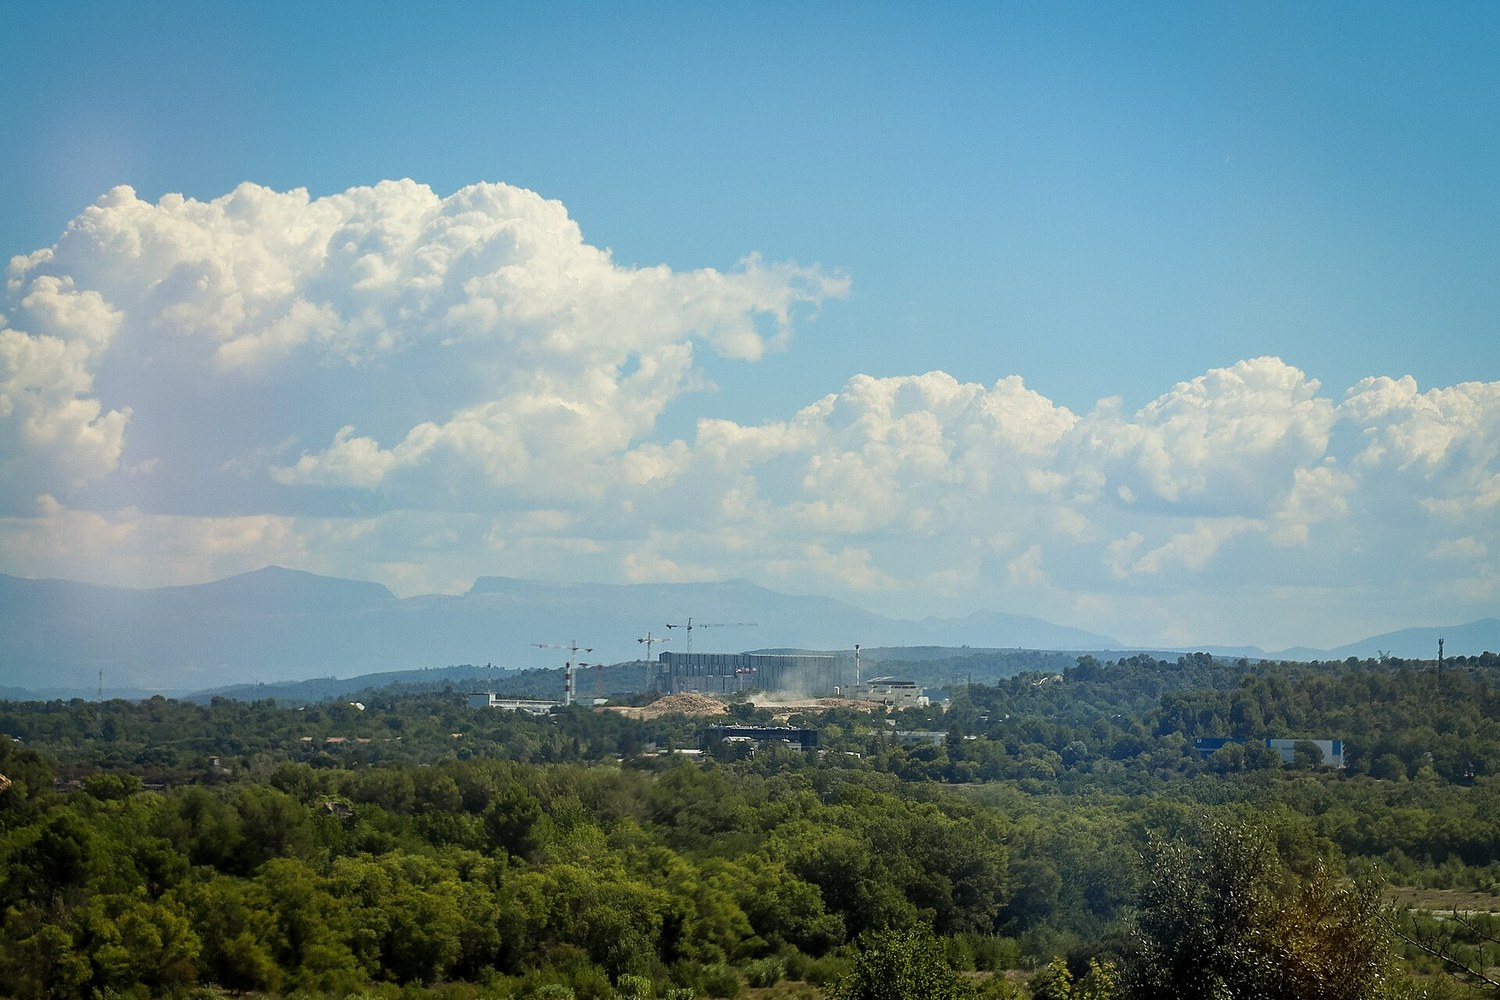
\includegraphics[width=0.78\textwidth]{../figures/z_iter_construction.jpg}
\caption{ITER 建设现场：主机厂房、电源与冷却系统在同一个场址上排开。聚变堆工程要算的电功率、可用率与维护窗口，就写在这片工地的总平面里。}
\label{fig:photo-appz3}
\figsource{Johannes Reimer，CC BY 4.0（Wikimedia Commons）}
\end{figure}

\section{可用率与年发电量：工程增益的另一半}
\label{sec:app-z-availability}

到 Z.5 为止算的都是「堆在运行的时候」的功率。但电站是卖给电网的，
电网只认\textbf{年发电量}：
\begin{equation}
E_{\mathrm{year}} = P_{\mathrm{net}}\times 8760\ \mathrm{h}\times A,
\label{eq:app-z-eyear}
\end{equation}
其中 $A$ 是可用率。取 $A=0.75$（\textbf{声明}值，含换包层与计划检修）：
\begin{equation}
E_{\mathrm{year}} = 5.14647\times10^{15}\ \mathrm{J} = 1429.6\ \mathrm{GWh},
\label{eq:app-z-eyearnum}
\end{equation}
折合标煤 $0.48606$ 百万吨（按 $0.34\ \mathrm{kg}$ 标煤/$\mathrm{kWh}$ 的\textbf{声明}口径）。
把可用率从 $0.75$ 提到 $0.85$：
\begin{equation}
\frac{\Delta E}{E} = \frac{0.85-0.75}{0.75} = 13.333\%,
\qquad
E_{\mathrm{year}}^{(0.85)} = 1620.2\ \mathrm{GWh}.
\label{eq:app-z-gain85}
\end{equation}
\textbf{十个百分点的可用率，换来 $13.333\%$ 的年发电量}。比在等离子体侧
抠 $13\%$ 的增益容易得多。这就是「工程增益的另一半」：
聚变功率决定上限，可用率决定实际拿到多少。

\begin{table}[htbp]
\centering
\small
\caption{可用率与年发电量。第四行是本节的结论：
\textbf{在工程侧提高可用率，往往比在等离子体侧提高增益更划算}。}
\label{tab:app-z-availability}
\begin{tabular}{p{3.4cm}p{3.2cm}p{3.2cm}p{3.3cm}}
\toprule
量 & 数值 & 由什么决定 & 含义 \\
\midrule
可用率 & $0.75$ & 声明值 & 含换包层与检修 \\
年发电量 & $1429.6\ \mathrm{GWh}$ & $P_{\mathrm{net}}\times8760\,\mathrm{h}\times A$ & $5.14647\times10^{15}\ \mathrm{J}$ \\
年停机 & $2190\ \mathrm{h}$ & $8760\times(1-A)$ & 一年四分之一停着 \\
可用率提到 $0.85$ & $1620.2\ \mathrm{GWh}$ & 同上 & 增幅 $13.333\%$ \\
折合标煤 & $0.48606$ 百万吨 & $0.34\ \mathrm{kg/kWh}$ & 声明口径 \\
\bottomrule
\end{tabular}

\end{table}

\begin{tip}{可用率是「另一半增益」}{tip-app-z-availability}
等离子体侧的所有努力（提高 $Q$、提高 $\beta$、抑制破裂）最终都只体现在一个数上：
$P_{\mathrm{net}}$。而年发电量还要乘 $A$。两者的地位完全对称。
\textbf{把 $A$ 从 $0.75$ 提到 $0.85$ 与把 $P_{\mathrm{net}}$ 提高 $13.333\%$ 等价}。
工程上后者常常更便宜，因为可用率取决于\textbf{维护方案}而不是等离子体物理。
\end{tip}

{\footnotesize
\textbf{出处：}可用率与年发电量的账参照 Freidberg \emph{Plasma Physics and Fusion
Energy}（2007，第 14 章）。
标煤折算系数是\textbf{声明的}量级口径（本书只用作对照，
不参与任何推导）。
}

\section{估算练习}
\label{sec:app-z-problems}

\textbf{练习 1} 若包层能量倍增从 $1.15$ 提到 $1.30$，$P_{\mathrm{th}}$、$P_{\mathrm{gross}}$、
$P_{\mathrm{net}}$ 各变成多少？$P_{\mathrm{net}}$ 涨了百分之多少？

\textbf{练习 2} 若热效率从 $0.40$ 提到 $0.45$，$P_{\mathrm{net}}$ 变成多少？涨幅是多少？

\textbf{练习 3} 若第一壁面积加倍（装置更大、或加装限流器），中子壁负载变成多少？
壁负载余量变成多少倍？

\textbf{练习 4} 若要求把中子通量衰减到 $10^{-8}$，屏蔽层需要多厚？比 $10^{-6}$ 的情形厚多少米？

\textbf{练习 5} 若 TBR 只做到 $1.05$，氚的净增量是多少？与 $1.10$ 的情形差多少？

\textbf{练习 6} 若可用率提到 $0.85$，年发电量是多少 GWh？增幅多少？折合标煤多少百万吨？

\textbf{解答 1} $P_{\mathrm{th}} = 1.30\times556.5 = 723.45\ \mathrm{MW}$，
$P_{\mathrm{gross}} = 0.40\times723.45 = 289.38\ \mathrm{MW}$，
$P_{\mathrm{net}} = 0.85\times289.38 = 245.97\ \mathrm{MW}$，是原来的 $1.1304$ 倍。
\textbf{要点}：$M$ 每提高 $0.15$，整链净电涨 $13\%$。因为它是乘法链最上游的因子。

\textbf{解答 2} $P_{\mathrm{gross}} = 0.45\times639.97 = 287.99\ \mathrm{MW}$，
$P_{\mathrm{net}} = 0.85\times287.99 = 244.79\ \mathrm{MW}$，涨幅 $12.5\%$。
\textbf{要点}：热效率提高 $5$ 个百分点（相对 $12.5\%$）就把净电带动 $12.5\%$。
\textbf{热机与包层一样是「一等公民」}，不是配套设备。

\textbf{解答 3} $q_n = 445.2/(2\times489.532) = 0.45472\ \mathrm{MW\,m^{-2}}$，
余量 $2/0.45472 = 4.3983$ 倍。\textbf{要点}：壁负载与面积成反比，
面积加倍余量也加倍；但装置尺寸是有限资源，所以真正的出路是提高
$P_n$ 的利用率而不是无限放大第一壁。

\textbf{解答 4} $x = 0.15\ln(10^{8}) = 2.7631\ \mathrm{m}$，
比 $10^{-6}$ 的情形厚 $0.69078\ \mathrm{m}$。\textbf{要点}：指数衰减意味着
\textbf{多挡两个数量级只多要 $0.69078\ \mathrm{m}$}。屏蔽的「边际成本」是对数级的，
这正是屏蔽设计可以做得很从容的原因。

\textbf{解答 5} $\Delta\dot m = 0.05\times31.191 - 0.11252 = 1.447\ \mathrm{kg\,year^{-1}}$，
比 $\mathrm{TBR}=1.10$ 时的 $3.0066\ \mathrm{kg\,year^{-1}}$ 少了一半多。
\textbf{要点}：TBR 从 $1.10$ 降到 $1.05$，净增从 $3.0066$ 掉到 $1.447\ \mathrm{kg\,year^{-1}}$，
但\textbf{仍然自持}。因为自持下限只有 $1.0036$。

\textbf{解答 6} $E_{\mathrm{year}} = 1620.2\ \mathrm{GWh}$，增幅 $13.333\%$，
折合标煤 $0.55086$ 百万吨。\textbf{要点}：与练习 2 的热效率改善幅度几乎相同，
但可用率的改善\textbf{不要求等离子体性能更好}。这是工程侧最「便宜」的增益。

\section{来源、分级与版权说明}
\label{sec:app-z-source}

\begingroup\small
本附录按难度分三档：Z.1 与 Z.2 是账本与判据，Z.3 与 Z.4 是两个子系统，
Z.5 与 Z.6 是工程收尾。练习 1--6 只需要本附录的公式与表，不需要查外部数据。

\begin{table}[htbp]
\centering
\small
\caption{本附录的借鉴来源与对应位置。只借鉴物理结论、公式形式与题型；
全部数值、表格与文字自拟并由仓库脚本复算。}
\label{tab:app-z-source}
\begin{tabular}{p{3.4cm}p{5.6cm}p{3.6cm}}
\toprule
本附录内容 & 借鉴来源 & 在本书里的位置 \\
\midrule
四步能量链与整链效率 &
Freidberg \emph{Plasma Physics and Fusion Energy}（2007）第 13、14 章 &
本附录 Z.1；附录 U \\
包层能量倍增与再循环份额 &
ITER 设计报告（1999）\emph{Nucl.\ Fusion} \textbf{39}, 2137 &
本附录 Z.1、Z.2 \\
中子壁负载、dpa 与包层寿命 &
Stacey \emph{Fusion Plasma Physics}（2005）第 1 章；Atzeni \& Meyer-ter-Vehn（2004）第 1 章 &
本附录 Z.2；附录 N 的第一壁口径 \\
氚增殖比、库存与自持 &
Freidberg（2007）第 14 章；ITER 氚系统设计报告（1999） &
本附录 Z.3；附录 N 的氚滞留账 \\
屏蔽衰减与低温制冷代价 &
Stacey（2005）第 1 章；Wesson \emph{Tokamaks}（第 4 版，2011）第 1 章 &
本附录 Z.4 \\
可用率与年发电量 &
Freidberg（2007）第 14 章 &
本附录 Z.6 \\
\bottomrule
\end{tabular}

\end{table}

版权与复现口径，四条：第一，\textbf{不复制}任何教材或论文的表格数值，
表 \ref{tab:app-z-chain} 到表 \ref{tab:app-z-source} 的每一个数字都由
\texttt{tools/\allowbreak{}calc/\allowbreak{}appZ\_calc.py} 在给定工作点上现算；

第二，\textbf{不复制}原书的题面与解答文字，
练习 1--6 的题目与解答均为本书自拟；

第三，\textbf{不复制}无法核验的 DOI 编号，
一律只给书名、作者、年份、卷期页；

第四，\textbf{不复制}任何未经复算的「精确值」。
凡本附录引入的\textbf{声明值}（包层倍增 $1.15$、热效率 $0.40$、再循环份额 $0.15$、
中子壁负载上限 $2\ \mathrm{MW\,m^{-2}}$、dpa 系数 $5$、包层寿命 $50\ \mathrm{dpa}$、
TBR $1.10$、氚半衰期 $12.32$ 年、库存 $2\ \mathrm{kg}$、处理循环 $4\ \mathrm{h}$、
屏蔽衰减长度 $0.15\ \mathrm{m}$、可用率 $0.75$、冷却剂比热 $5.2\ \mathrm{kJ\,kg^{-1}K^{-1}}$、
温升 $200\ \mathrm{K}$、泵份额 $0.01$、制冷 COP $300$、标煤系数 $0.34\ \mathrm{kg/kWh}$）
都在正文里写明是量级值，不假装精确。

\begin{tip}{把「声明值」列成一张清单}{tip-app-z-honest}
本附录引入的声明值有十七个。比附录 X、Y 都多，因为工程参数天然依赖设计选型。
与其把它们散落在正文里，不如在 Z.8 末尾\textbf{一次列全}（见上）。
这样读者一眼就能分清\textbf{哪些数是本书从第一原理算的、哪些是本书声明的}。
附录 V 立下的这条口径，这里是第四次使用：\textbf{把做不到的地方标出来，
比用一个看起来精确的数字盖过去更有用}。
\end{tip}
\endgroup
